
\documentclass[submit]{harvardml}

% Put in your full name and email address.
\name{Your Name}
\email{email@fas.harvard.edu}

% List any people you worked with.
\collaborators{%
  John Doe,
  Fred Doe
}

% You don't need to change these.
\course{CS181-S16}
\assignment{Assignment \#4}
\duedate{5:00pm Feb 1, 2016}

\usepackage[OT1]{fontenc}
\usepackage[colorlinks,citecolor=blue,urlcolor=blue]{hyperref}
\usepackage[pdftex]{graphicx}
\usepackage{subfig}
\usepackage{fullpage}
\usepackage{palatino}
\usepackage{mathpazo}
\usepackage{amsmath}
\usepackage{amssymb}
\usepackage{color}
\usepackage{todonotes}
\usepackage{listings}
\usepackage{common}
\usepackage{bm}

\usepackage[mmddyyyy,hhmmss]{datetime}

\definecolor{verbgray}{gray}{0.9}

\lstnewenvironment{csv}{%
  \lstset{backgroundcolor=\color{verbgray},
  frame=single,
  framerule=0pt,
  basicstyle=\ttfamily,
  columns=fullflexible}}{}

\begin{document}
\begin{center}
{\Large Homework 4: Clustering}\\
\end{center}

There is a mathematical component and a programming component to this homework.
Please submit ONLY your PDF to Canvas, and push all of your work to your Github
repository. If a question requires you to make any plots, please
include those in the writeup.


%%%%%%%%%%%%%%%%%%%%%%%%%%%%%%%%%%%%%%%%%%%%%
% Problem 1
%%%%%%%%%%%%%%%%%%%%%%%%%%%%%%%%%%%%%%%%%%%%%
\begin{problem}[The Curse of Dimensionality, 4pts]
In~$d$ dimensions, consider a hypersphere of unit radius, centered at zero,
which is inscribed in a hypercube, also centered at zero, with edges of length
two.  What fraction of the hypercube's volume is contained within the
hypersphere?  Write this as a function of~$d$.  What happens when~$d$ becomes
large?
\end{problem}
\subsection*{Solution}


\newpage
\begin{problem}[Norms, Distances, and Hierarchical Clustering, 5 pts]

  Consider the following four data points, belonging to three clusters: the
  black cluster $((x_1, y_1) = (0.1, 0.5) $ and $(x_2, y_2) = (0.35, 0.75))$,
  the red cluster $(x_3, y_3) = (0.28, 1.35)$ cluster, and the blue cluster
  $(x_4, y_4) = (0, 1.01)$.

  \begin{center} 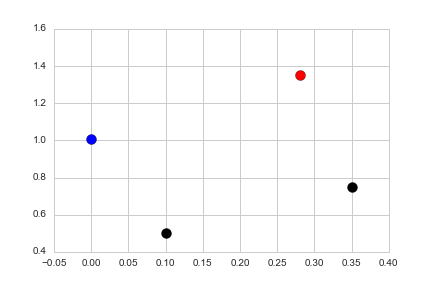
\includegraphics[scale=.4]{scatterplot.png} \end{center}
  At each step of hierarchical clustering, the two most similar (or least
  dissimilar) clusters are merged together. This step is repeated until there is
  one single group. Different distances can be used to measure group
  dissimilarity. Recall the definition of the $l_1$, $l_2$, and $l_{\infty}$
  norm:
  \begin{itemize}
    \item For $\mathbf{x} \in \mathbb{R}^n, \| \mathbf{x} \|_1 = \sum_{i = 1}^n
      |x_i|$
    \item For $\mathbf{x} \in \mathbb{R}^n, \| \mathbf{x} \|_2 = \sqrt{\sum_{i =
      1}^n x_i^2 }$
    \item For $\mathbf{x} \in \mathbb{R}^n, \| \mathbf{x} \|_{\infty} = \max_{i
      = 1}^n |x_i|$
  \end{itemize}
  Also recall the definition of single-link distance, complete-link distance,
  and average-link distance between two clusters:
  \begin{itemize}
    \item Single-link clustering: for clusters $G$ and $H$, $d_{S}(G, H) =
    \min_{i \in G, j\in H} d(i, j)$
    \item Complete-link clustering: for clusters $G$ and $H$, $d_{C}(G, H) =
    \max_{i \in G, j\in H} d(i, j)$
    \item Average-link clustering: for clusters $G$ and $H$, $d_{A}(G, H) =
      \frac{1}{|G| |H|} \sum_{i\in G}\sum_{j \in H} d(i, j)$
  \end{itemize}
  \paragraph{Warm up question.} \noindent Draw the 2D unit sphere for each norm,
  defined as $\mathcal{S} = \{x \in \mathbb{R}^2: \|x\| = 1 \}$. Feel free to do
  it by hand, take a picture and include it in your pdf.

  \paragraph{Main question.}
  \noindent For each norm ($l_1, l_2, l_\infty$) and each clustering method
  (single, complete, or average link clustering), specify which 2 clusters would
  be the first to merge.
\end{problem}
\subsection*{Solution}

\newpage

\section*{K-Means [15 pts]}
Implement K-Means clustering from scratch.\footnote{That is, don't use a
third-party machine learning implementation like \texttt{scikit-learn};
\texttt{numpy} is fine.}. You have been provided with the MNIST dataset. You can
learn more about it at  \url{http://yann.lecun.com/exdb/mnist/}. The MNIST task
is widely used in supervised learning, and modern algorithms with neural
networks do very well on this task. We can also use MNIST for interesting
unsupervised tasks. You are given representations of 6000 MNIST images, each of
which are $28\times28$  handwritten digits. In this problem, you will implement
K-means clustering on MNIST, to show how this relatively simple algorithm can
cluster similar-looking images together quite well.

\begin{problem}[K-means, 15pts]
The given code loads the images into your environment as a 6000x28x28 array.
Implement K-means clustering on it for a few different values of $K$, and show
results from the fit. Show the mean images for each class, and by selecting a
few representative images for each class. You should explain how you selected
these representative images. To render an image, use the numpy imshow function,
which the distribution code gives an example of. Use squared norm as your
distance metric. You should feel free to explore other metrics along with
squared norm if you are interested in seeing the effects of using those. Also,
your code should use the entire provided 6000-image dataset (which, by the way,
is only 10\% of the full MNIST set).

Are the results wildly different for different restarts and/or different $K$?
Plot the K-means objective function as a function of iteration and verify that
it never increases.

Finally, implement K-means++ and see if gives you more satisfying
initializations (and final results) for K-means. Explain your findings.

As in past problem sets, please include your plots in this document. There may
be tons of plots for this problem, so feel free to take up multiple pages, as
long as it is organized.
\end{problem}
\subsection*{Solution}


%Figure out how to load it into your environment and turn it into a set of
%vectors.  Run K-Means on it for a few different~$K$ and show some results from
%the fit.  What do the mean images look like?  What are some representative
%images from each of the clusters?  Are the results wildly different for
%different restarts and/or different~$K$?  Plot the K-Means objective function
%(distortion measure) as a function of iteration and verify that it never
%increases.

%\subsection*{4. Implement K-Means++ [4 pts]} mplement K-Means++ and see if it
%gives you more satisfying initializations for K-Means.  Explain your findings.

\newpage
\begin{problem}[Calibration, 1pt]
Approximately how long did this homework take you to complete?
\end{problem}


\end{document}
